\section{Evaluation}
\label{sec:evaluation}
The performance of MCRP is compared against the standard ContikiMAC with RPL. We analyse MCRP using an end-to-end packet delivery performance metric.

\subsection{Experimental Setup}
We evaluate the protocol in the  Cooja simulated environment with emulation of TMote sky nodes that feature the CC2420 transceiver, a 802.15.4 radio. The nodes run on IPv6, using UDP with standard RPL and 6LoWPAN protocols. The network consists of 31 nodes which are used to run the simulation where we have 1 border router node, 16 interference nodes, and 14 duty cycled nodes that act as UDP clients to send packets to LPBR spanning over 20-30 metres between each node. RPL border router is used as LPBR in order to move most processing decisions on a PC as it has more RAM and better processing capabilities than a sensor. TelosB has limited RAM and ROM of 10K bytes and 48K bytes of flash memory \cite{telosb-datasheet}. By using a border router, this allows channel changing to be decided in real time without draining the memory and battery on a sensor. The border router also acts as the root of the tree.

We simulated a controlled interference node that generates semi-periodic bursty interference to resemble a simplified Wi-Fi or Bluetooth transmitter on several channels at random. We use the interference model proposed in \cite{Boano:2010:MSM:2127940.2127963}. The interference has two states, a clear state and an interference state. 
In the interference state, the interference node generates packets for a time that is uniformly distributed between $9/16$ seconds and $15/16$ seconds. In the clear state the interferer produces no packets and stays in this state for between $3/4 * \emph{clear\textunderscore time}$ and $5/4 * \emph{clear\textunderscore time}$ where \emph{clear\textunderscore time} refers to the rate of interference.
We use multiple channels interference in our simulation to show our hypothesis that our multichannel protocol can help avoid interference. We consider the scenario where ContikiMAC with RPL system is subject to interference on its channel after set up has successfully completed so the RPL set up is allowed to complete before interference begins.

We use an end-to-end packet delivery performance metric to evaluate MCRP. The transmission success rate is calculated from the sender to the receiver over multiple hops. We also look at the loss over time to observe the protocol performance in the presence of interference. We considered two multiple channels interference scenarios; (1) extreme and no interference rate on 8 channels each and (2) extreme, moderate, mild and no interference rate on 4 channels each. The interference channels are randomly chosen from the available 16 channels and the same interference channels and rates are used throughout the experiments. However, channel 26 is kept clear from interference in order to ensure RPL set up is unaffected. In scenario 1, we fixed the interference rate to extreme and no interference to observe the effect it has on channel changing decisions. In scenario 2, we vary the interference rate to observe how MCRP copes in deciding a channel when there is more interference than scenario 1 but with less interference intensity. 

We run the simulation for a duration of 45-60 minutes to send 210-560 packets. When the nodes are switched on for the first time, all nodes are initialised to channel 26, the default channel for Contiki MAC layer. RPL is allowed five minutes to set up (which is ample time). RPL topology is formed in a minute. We wait for another five minutes to allow trickle timer to double the interval length so that RPL control messages are not being sent frequently. We then let our multichannel protocol runs for 25 minutes. In our 15 nodes simulation, our protocol takes 20-25 minutes to run the channel change set up. We allow another 5 minutes wait time if retransmissions happen. 
In a single channel simulation, all the nodes are changed to channel 22 after 5 minutes of RPL set up time. This allows RPL to have enough time to discover all nodes to form an optimised topology. The topology formation does not form completely if the interference node interferes from the beginning. The interference node starts sending packets to interfere after 3 minutes the system is switched on so that the interference channel is involve in the channel changes decision. We proved that our protocol tries to avoid changing to the interference channel through time out and probing failures. After 30 minutes, the client nodes will send a normal packet periodically every 30-60 seconds to LPBR. This is done in order to avoid collision of the nodes sending at the same time. 

The simulations are repeated ten times. In all plots, the mean value of the ten simulations is plotted with error bars corresponding to one standard deviation in either deviation to give a measure of repeatability. The plots are of the proportion of received packets (from 0\% to 100\%) against time where the loss is measured over the previous time period.  The x-value is shifted slightly left and right to prevent error bars overlapping.

\subsection{Packet loss rates with single channel RPL versus multi-channel}
The performance obtained in ContikiMAC with RPL (single channel) is compared with our protocol in terms of packet loss rate.
As described previously, levels of interference used (referred to as \emph{clear\textunderscore time} in \cite{Boano:2010:MSM:2127940.2127963})
vary between 100\% (no interference), 75\% (mild), 50\% (moderate) and 25\% (extreme) where the percentage is the ratio of the time the channel is clear for transmission.  All our tests have a common format: the RPL procedure is allowed to set up without interference in order not to bias subsequent tests.
Then the interferers begin to operate with a constant level (none, mild, moderate or extreme).

\begin{figure}
\centering
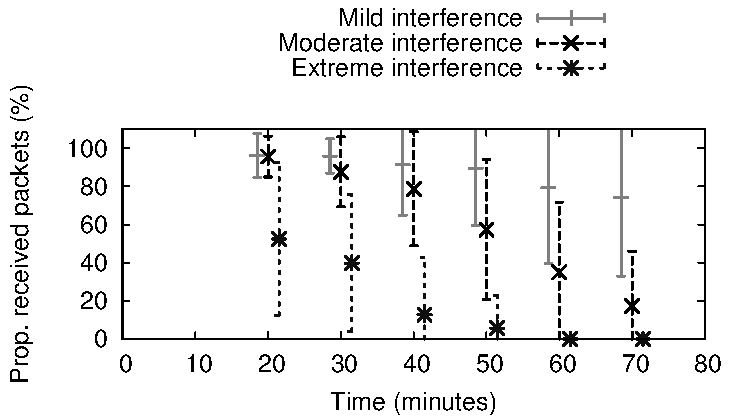
\includegraphics[width=0.45\textwidth]{experiments/single_channel.pdf}
\caption{Level of packet loss for mild, moderate and extreme interference levels using single channel}
\label{fig:interference}
\end{figure}

\begin{figure}
\centering
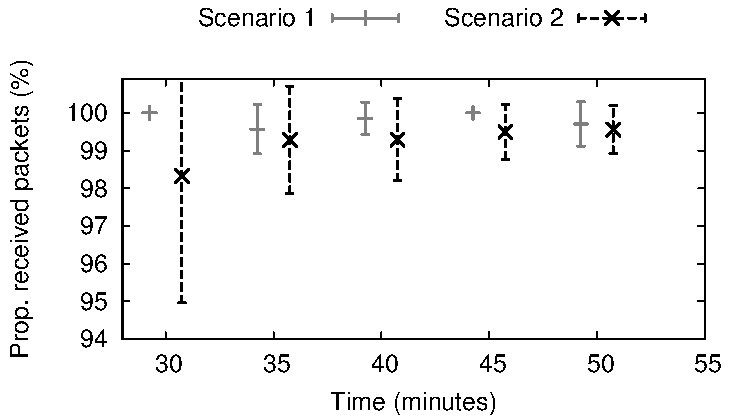
\includegraphics[width=0.45\textwidth]{experiments/multi_channel.pdf}
\caption{Level of packet loss for scenario 1 and scenario 2 using multi channel}
\label{fig:multi_interference}
\end{figure}

Figure \ref{fig:interference} shows the results for ContikiMAC with RPL protocol. It can be seen that the level of packet loss varies considerably between experiments (the error bars are always large). It can also be seen that even for mild interference there is considerable loss and this gets worse as time proceeds. In the extreme interference case the loss always goes up until no packets are received. For mild interference the system evolves until it is losing around 20\% of packets but this can increase.

For our new multiple channel protocol we consider two interference scenarios.
In scenario 1 half the channels (including the original channel) have no
interference at all and half the channels have extreme interference.
In scenario 2, four channels (including the original channel) have no
interference, four have mild, four moderate and four extreme interference.
Figure \ref{fig:multi_interference} shows multi channel results for these
two scenarios.  In scenario 1 the protocol performs extremely well, the packet loss is near zero and the protocol successfully detects channels with interference.
Scenario 2 has similar results as in scenario 1. The protocol does well at reducing the effects of interference and could detect moderate and mild interference.

In MiCMAC \cite{micmac}, it is stated that MiCMAC has a transmission success rate of 99\% when using four channels. However, when more than four channels are used (8 or 16 channels), MiCMAC performance degrades to approximately 88\% (16 channels) due to interference channels. The interference model that MiCMAC uses is different than ours. They compare the result with Chrysso where Chrysso has a transmission success rate of approximately 88\% for 4 and 8 channels and suffers greatly in the case of 16 channels with 60\% success rate.
Our protocol on the other hand, shows greatly reduced loss rate with any number of channels at approximately 99\%.

\subsection{Setup Overhead}
Obviously the system of changing channels and probing to see if a channel is free of interference introduces a certain amount of overhead into
the protocol. This takes the form of (a) extra messages passed and (b) extra time taken to set up. Default RPL on ContikiMAC for the topology considered in these experiments completed its set up using 276 packets. Our multi-channel protocol completed its set up in 716 packets, that is an overhead of 440 packets on top of RPL. 
This overhead comes from the channel changing messages to nodes and neighbours, probing messages, channel confirmation messages and acknowledgement packets which are required to ensure a thorough channel change decision.
However, it is worth mentioning that this is a one-off cost. This represents (in this experimental set up) approximately one hour of extra packets in the situation of a deployment that is meant to work for weeks or months.  In terms of set up time, our protocol begins to change channels only when the RPL set up process is complete (or at least stabilises). The set up time is 1154 seconds beyond the RPL set up time of 286 seconds. However, it should be noted that, in fact, our system remains fully functional and capable of sending packets during the set up so this set up overhead does not matter to data transmission.
Therefore we conclude that data sending costs (extra packets) of set up are negligible in the context of a deployment that will last more than a day. The extra set up time is also negligible within this context and furthermore does not degrade performance of the network during this set up phase.